\pagestyle{plain} % No headers, just page numbers

\chapter{\uppercase {Hierarchical DeepPruner: A Novel Framework for Search Space Reduction}}

As graph instances grow to millions of nodes, even a lightweight sequential algorithm
faces scalability challenges, particularly for problems where calculating marginal gain
is \#P-hard. At the same time, existing learning-based pruning methods achieve fast
inference but demand problem-specific domain knowledge for algorithm design, making them
difficult to apply to new CO problems. In this chapter, we introduce Hierarchical
DeepPruner (H-DeepPruner)~\cite{nath2025hdeeppruner}, an adaptive two-stage framework
that combines supervised learning with reinforcement learning for search space reduction
under size constraints. The first stage uses a graph neural network to quickly eliminate
vertices unlikely to be part of the solution, without requiring any hand-crafted features
or domain knowledge. The second stage applies a tree search procedure to further refine
the pruned ground set by considering interdependencies among elements.

\begin{figure}[t]
  \centering
  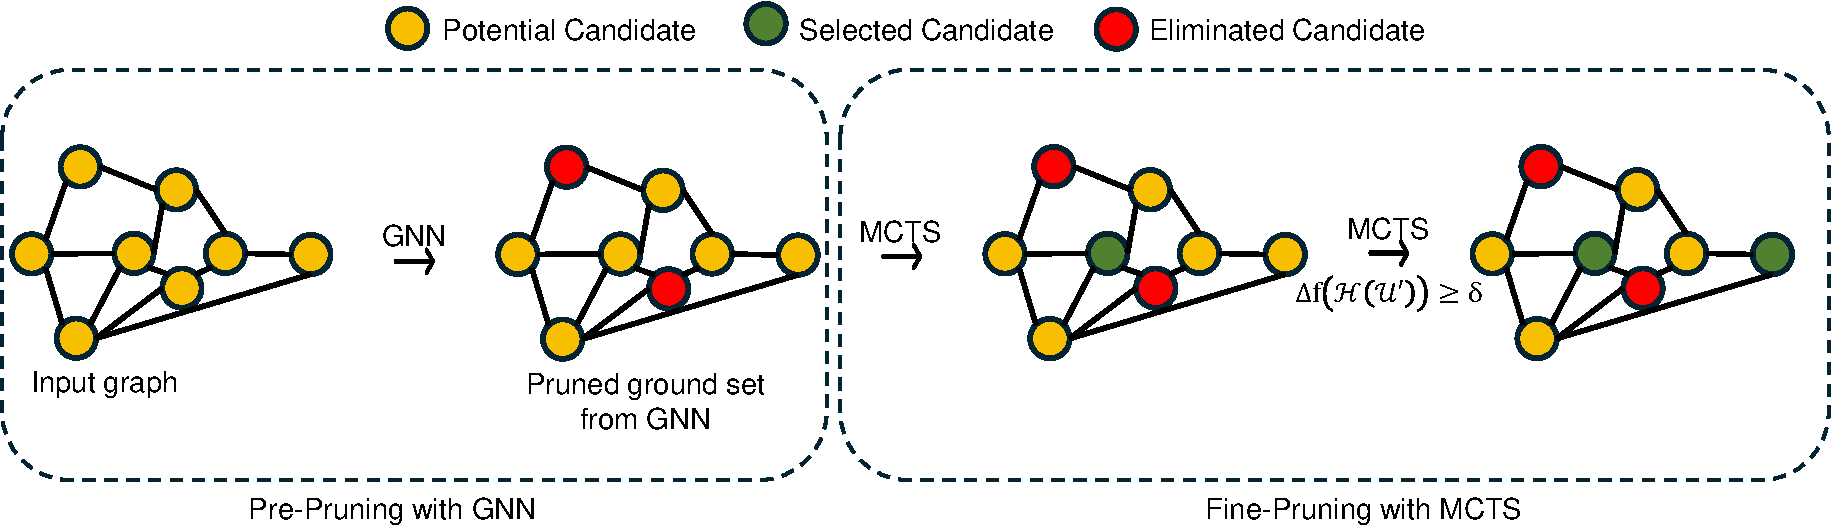
\includegraphics[width=0.9\textwidth]{figures/hdeeppruner/framework.pdf}
  \caption{Illustration of the H-DeepPruner framework. The process begins with a GNN
    discarding elements unlikely to contribute to an optimal solution. MCTS then
    iteratively constructs a much smaller ground set with progressive deepening.}
  \label{fig:hdp-framework}
\end{figure}

\section{Problem Setting}

We consider the same pruning problem as in Chapter~3, restricted to size constraints.
Given a ground set $\mathcal{U}$ and an exact method $\mathcal{OPT}$, an optimal solution
is defined as $X^\star = \arg\max_{X \subset \mathcal{U}, |X| \leq B} f(X)$. The goal is
to find a significantly smaller ground set $\mathcal{U}'$ with
$|\mathcal{U}'| \ll |\mathcal{U}|$ while preserving the objective value, i.e.,
$f(\mathcal{OPT}(\mathcal{U}')) / f(\mathcal{OPT}(\mathcal{U})) = 1$. The motivating
question is: \emph{Is it possible to develop a pruning algorithm that does not rely on
domain-specific knowledge or feature engineering, yet remains practical and competitive
with existing heuristics?}

\section{Method}

H-DeepPruner is schematically illustrated in Figure~\ref{fig:hdp-framework}. It consists
of two main stages: an initial pruning step using a GNN, followed by Neural Monte Carlo
Tree Search (NMCTS) for further reduction. The key insight behind this hierarchical
design is that each stage addresses a different aspect of the pruning problem. The GNN
performs a fast, coarse-grained pruning by classifying each node independently --- it
can quickly eliminate a large number of clearly irrelevant nodes (e.g., low-degree
peripheral nodes in influence maximization) but cannot reason about redundancy among
the retained nodes. NMCTS then performs a slower, fine-grained refinement that accounts
for interdependencies between elements, constructing a compact ground set where each
retained element contributes meaningfully to the solution.

\subsection{Stage 1: Pre-Pruning with GNN}

The first stage introduces a GNN to eliminate nodes that are unlikely to be part of the
solution, allowing NMCTS to focus computational resources on promising nodes. This step
parallels the handcrafted degree heuristic in GCOMB~\cite{manchanda2020gcomb}, but
instead of relying on a manually designed heuristic, we hypothesize that vertices in the
optimal solution exhibit similar local structures that can be identified from local
neighborhood features alone.

We use a Graph Convolutional Network (GCN)~\cite{kipf2016semi}. Given an undirected graph
$G(V, E)$ with adjacency matrix $A$, the GCN updates node representations as:
\[
h_{v_i}^{(k)} = f_2^{(k)}\!\left(\left\{h_{v_i}^{(k-1)},\;
f_1^{(k)}\!\left(\left\{h_u^{(k-1)} : u \in N(v_i)\right\}\right)\right\}\right),
\]
where $N(v_i) = \{v_j \in V \mid A_{i,j} \neq 0\}$ is the set of neighbors of node
$v_i$, function $f_1^{(k)}$ aggregates feature information over the set of neighboring
nodes, and function $f_2^{(k)}$ combines the node's own hidden features from iteration
$(k-1)$ with the aggregated neighborhood features. We empirically find that GCN,
which retains full neighborhood information, outperforms GraphSAGE, which samples a
fixed-size subset of neighbors.

\textbf{Random Node Initialization.} Instead of using hand-crafted features, we adopt
random node initialization~\cite{abboud2020surprising}, where node features are set as
$h_{v_i}^{(0)} \sim U(0,1)$. The hypothesis is that vertices in the optimal solution
exhibit similar local structures, identifiable from local neighborhood features alone.
This eliminates the need for problem-specific features such as eigenvector centrality
(used by LeNSE~\cite{ireland2022lense}) or Fourier Feature Mapping (used by
COMBHelper~\cite{tian2024combhelper}).

\textbf{Training.} Training data is generated from Erd\H{o}s-R\'{e}nyi (ER) random
graphs~\cite{erdos1960evolution}. Each graph is solved with a heuristic to obtain the
optimal ground set.
The GNN is trained with weighted cross-entropy loss to prevent non-solution vertices from
dominating training, with balanced sampling from solution and non-solution sets each
epoch.

\textbf{Inference.} At test time, we simply discard vertices the GNN predicts are
unlikely to be in the solution in a single pass. The GNN can remove a large number of
elements without compromising objective value.

\subsection{Stage 2: Fine-Pruning with Neural Monte Carlo Tree Search}

While the GNN can prune a large number of elements, the pruned ground set is still many
times larger than the budget. Moreover, the GNN predicts membership independently per
node, potentially retaining redundant elements. To address this, we introduce a Neural
MCTS (NMCTS) stage that constructs a solution from scratch, considering dependencies
among elements.

We formulate the pruning process as a Markov Decision Process (MDP), where the goal is
to sequentially build up a pruned ground set by adding one element at a time. Formally:
\begin{itemize}
  \item \textbf{State} $s$: the current pruned ground set together with potential
    candidates for addition (i.e., the remaining elements from the GNN-pruned set).
  \item \textbf{Action}: selecting an element from the candidates and adding it to the
    pruned ground set.
  \item \textbf{Transition}: the state is updated with the newly expanded pruned ground
    set and the selected element is removed from the candidate pool.
  \item \textbf{Reward}: the objective value obtained by running the downstream heuristic
    on the current pruned ground set. This directly measures how well the pruned set
    supports finding high-quality solutions.
  \item \textbf{Terminal condition}: a fixed number of elements have been added to the
    pruned ground set.
\end{itemize}
This sequential formulation allows NMCTS to account for element interdependencies: at each
step, the algorithm evaluates how a candidate element complements the elements already
selected, rather than assessing each element in isolation as the GNN does.

Neural Monte Carlo Tree Search (NMCTS) integrates neural networks into MCTS to
efficiently explore and evaluate large decision spaces. MCTS operates by building a
search tree and simulating outcomes to estimate the value of actions. NMCTS guides this
process using a policy network and a value network, both sharing the same GCN backbone
architecture as the pre-pruning GNN.

NMCTS gradually constructs a solution starting from an empty set, adding one element at
a time. At each step, it evaluates the current pruned ground set, considering the elements
already selected and selecting elements that contribute to the current pruned ground set.
The child node is selected based on the Predictor + Upper Confidence Bound (PUCT)
formula:
\[
PUCT = Q(s,a) + c_{puct} \cdot P(s,a) \cdot
\frac{\sqrt{\sum_b N(s,b)}}{1 + N(s,a)},
\]
where $Q(s,a)$ is the average reward for taking action $a$ in state $s$, $P(s,a)$ is the
prior probability of selecting action $a$ as predicted by the policy network, $N(s,a)$ is
the visit count for the state-action pair, $\sum_b N(s,b)$ is the total visit count of
all actions at state $s$, and $c_{puct}$ is a hyperparameter that controls the balance
between exploration and exploitation.

MCTS operates in four phases (see Figure~\ref{fig:hdp-mcts}). In the
\textbf{selection} phase, the algorithm starts at the root node and successively selects
a child node until reaching one that is either terminal or unexpanded. In the
\textbf{expansion} phase, upon reaching a leaf node, the algorithm adds a new child node
by expanding the action with the highest prior probability as predicted by the policy
network. In the \textbf{simulation} phase, the newly expanded node is evaluated. If the
node is terminal, the true reward is returned. Otherwise, the algorithm uses a value
network to predict the expected reward from the state. Finally, in the
\textbf{backpropagation} phase, the simulation outcome is propagated up the tree to
update the statistics of all visited nodes, refining the estimates for future decisions.

\begin{figure}[t]
  \centering
  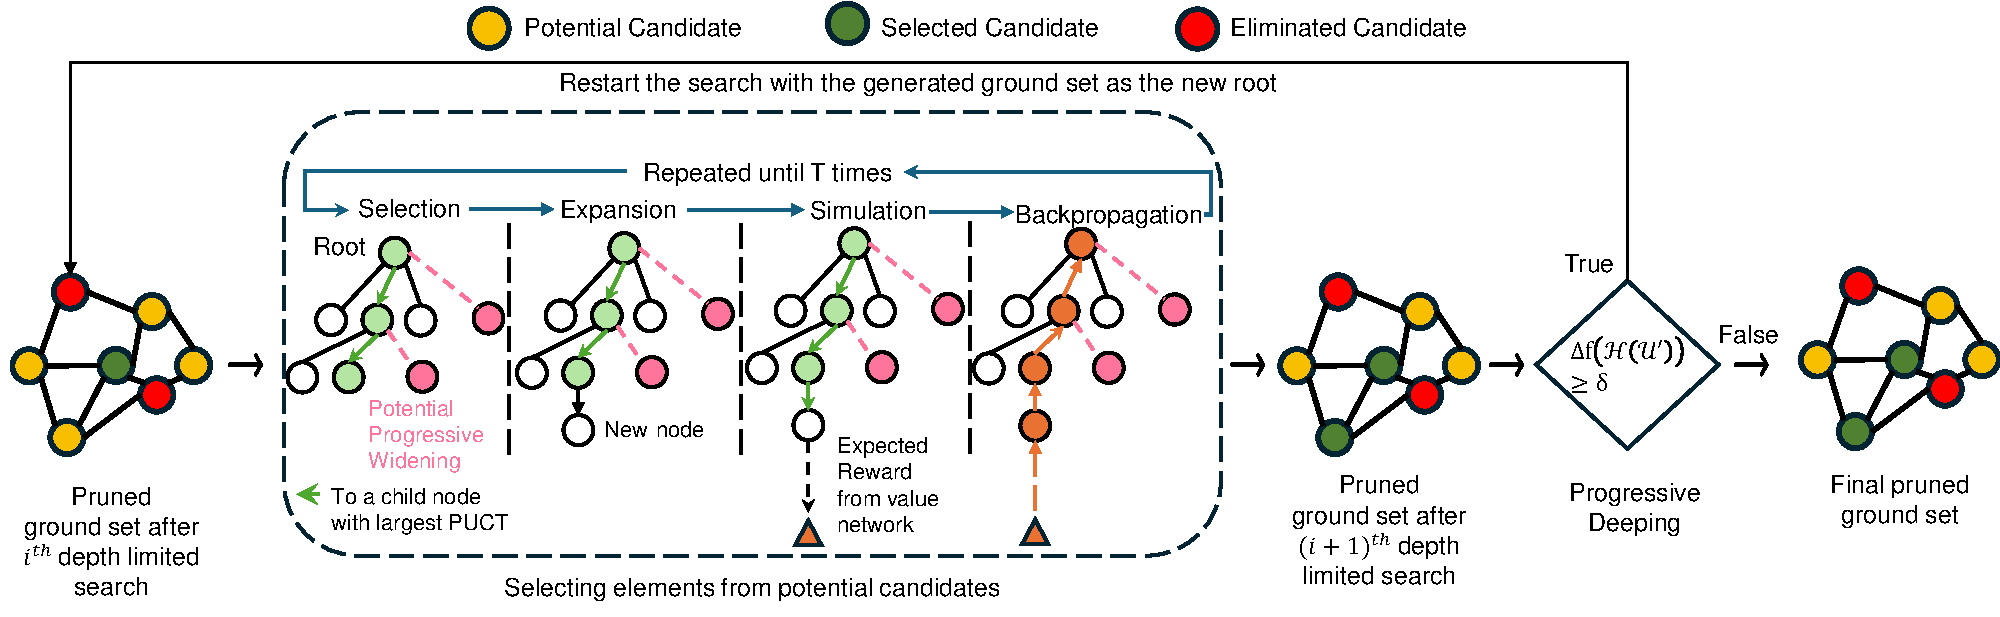
\includegraphics[width=0.9\textwidth]{figures/hdeeppruner/mcts.pdf}
  \caption{Illustration of MCTS with fixed depth and progressive widening for generating
    a pruned ground set. The search begins with an empty ground set and incrementally adds
    candidate elements. After each depth-limited search, progressive deepening checks
    whether the objective value improved sufficiently to continue.}
  \label{fig:hdp-mcts}
\end{figure}

\textbf{Progressive Widening.} During testing, the NMCTS is too slow especially for large
action spaces. As a result, the number of simulations becomes intractable. We apply
progressive widening~\cite{couetoux2011continuous}, which maintains a finite list of
child chance nodes to be searched and incrementally adds a new child chance node $N_c$ to
the list of child nodes of parent node $N_p$ based on the visitation counts. Specifically,
a new child node is added every time the following is satisfied:
$|\text{visits}(N_p)^\alpha| \geq |\text{CHILDREN}(N_p)|$,
where $\alpha \in (0,1)$ is a parameter that controls the growth rate. This allows
gradually increasing the number of choices or actions explored during the search process,
starting from a narrow focus and expanding it as more information is gained.

\textbf{Progressive Deepening.} We also introduce \emph{progressive deepening}, a search
strategy designed to refine the search space by iteratively expanding the search tree
based on improvements in the objective value. The search starts at the root node with an
empty subset and explores solutions up to a fixed depth. Initially, the objective value is
zero. Following each depth-limited search, the algorithm checks if there is a significant
improvement in the objective value compared to the previous search. If an improvement is
found, the search restarts from the root node using the current solution, effectively
deepening the search by focusing on promising areas. If, however, no significant
improvement is observed, signifying a potential plateau, the search terminates. This
method prevents the search tree from growing uncontrollably, as it focuses on expanding
only when progress is being made.

\section{Experimental Evaluation}

We compare H-DeepPruner to three state-of-the-art learning-based pruning methods across
three CO problems on graphs, following the experimental setup
of~\cite{ireland2022lense}.

\subsection{Experimental Setup}

\textbf{Applications.} We evaluate on three budget-constrained CO problems: Maximum Cover
(MaxCover), Maximum Cut (MaxCut), and Influence Maximization (IM) under the independent
cascade model with $p = 0.01$, all with budget $k = 100$.

\textbf{Datasets.} We use the same eight real-world graphs from
SNAP~\cite{leskovec2016snap} as in Chapter~3. Importantly, H-DeepPruner is trained on
ER graphs~\cite{erdos1960evolution} (not the SNAP training splits), unlike baselines which
train on the actual graph data.

\textbf{Baselines.} We compare against GCOMB~\cite{manchanda2020gcomb},
COMBHelper~\cite{tian2024combhelper}, and LeNSE~\cite{ireland2022lense}.

\textbf{Evaluation Metrics.} We use the same three metrics as in Chapter~3: pruning
approximation ratio $P_r$, pruned fraction $P_g$, and combined metric $C = P_r \cdot P_g$.
Additionally, we report speed-up
$S = \text{time}_{\mathcal{U}} / (\text{time}_{\mathcal{U}'} + \text{time}_{\text{prune}})$,
measuring the acceleration of heuristics on the pruned ground set.

\subsection{Results}

\begin{table}[t]
\centering
\caption{Size constraint results ($k = 100$) for H-DeepPruner: pruning approximation
  ratio $P_r$, pruned fraction $P_g$, and combined metric $C = P_r \cdot P_g$. Best $C$
  in bold; ``--'' indicates timeout. *Values as reported
  in~\cite{ireland2022lense}.}
\label{tab:hdp_size_constraint}
\resizebox{\textwidth}{!}{%
\begin{tabular}{@{}l ccc ccc ccc ccc@{}}
\toprule
& \multicolumn{3}{c}{H-DeepPruner} & \multicolumn{3}{c}{GCOMB*} & \multicolumn{3}{c}{COMBHelper} & \multicolumn{3}{c}{LeNSE*} \\
\cmidrule(lr){2-4}\cmidrule(lr){5-7}\cmidrule(lr){8-10}\cmidrule(lr){11-13}
Graph & $P_r$ & $P_g$ & $C$ & $P_r$ & $P_g$ & $C$ & $P_r$ & $P_g$ & $C$ & $P_r$ & $P_g$ & $C$ \\
\midrule
\multicolumn{13}{c}{\textbf{Maximum Cover}} \\
\midrule
Facebook  & 0.985 & 0.950 & \textbf{0.936} & 0.927 & 0.070 & 0.065 & 1.000 & 0.384 & 0.384 & 0.966 & 0.070 & 0.068 \\
Wiki      & 0.997 & 0.961 & \textbf{0.958} & 0.990 & 0.030 & 0.030 & 1.000 & 0.453 & 0.453 & 1.094 & 0.340 & 0.372 \\
Deezer    & 0.997 & 0.995 & \textbf{0.993} & 0.994 & 0.130 & 0.129 & 1.000 & 0.728 & 0.728 & 0.979 & 0.750 & 0.734 \\
Slashdot  & 0.990 & 0.997 & \textbf{0.987} & 1.000 & 0.020 & 0.020 & 1.000 & 0.984 & 0.984 & 0.979 & 0.690 & 0.676 \\
Twitter   & 0.972 & 0.997 & \textbf{0.969} & 0.997 & 0.170 & 0.170 & 1.000 & 0.565 & 0.565 & 0.989 & 0.330 & 0.326 \\
DBLP      & 0.969 & 0.999 & \textbf{0.969} & 0.999 & 0.030 & 0.030 & 1.000 & 0.182 & 0.182 & 0.990 & 0.900 & 0.891 \\
YouTube   & 0.997 & 1.000 & \textbf{0.997} & 0.998 & 0.070 & 0.070 & 1.000 & 0.957 & 0.957 & 0.982 & 0.790 & 0.776 \\
Skitter   & 0.959 & 1.000 & \textbf{0.959} & 0.999 & 0.100 & 0.100 & -- & -- & -- & 0.976 & 0.700 & 0.683 \\
\midrule
\multicolumn{13}{c}{\textbf{Maximum Cut}} \\
\midrule
Facebook  & 0.998 & \textbf{0.880} & \textbf{0.879} & 0.813 & 0.950 & 0.772 & 1.000 & 0.154 & 0.154 & 1.000 & 0.070 & 0.070 \\
Wiki      & 0.998 & 0.969 & \textbf{0.966} & 0.920 & 0.960 & 0.883 & 1.000 & 0.701 & 0.701 & 0.981 & 0.390 & 0.383 \\
Deezer    & 0.998 & 0.995 & \textbf{0.993} & 0.850 & 0.990 & 0.842 & 1.000 & 0.375 & 0.375 & 0.975 & 0.740 & 0.722 \\
Slashdot  & 1.000 & 0.997 & \textbf{0.997} & 0.632 & 0.990 & 0.626 & 0.794 & 0.993 & 0.788 & 0.990 & 0.620 & 0.614 \\
Twitter   & 0.974 & 0.997 & \textbf{0.971} & 0.628 & 0.990 & 0.622 & 1.000 & 0.554 & 0.554 & 0.987 & 0.480 & 0.474 \\
DBLP      & 0.964 & 0.999 & \textbf{0.963} & 0.646 & 0.990 & 0.640 & 1.000 & 0.183 & 0.183 & 0.993 & 0.920 & 0.914 \\
YouTube   & 0.981 & 1.000 & \textbf{0.981} & 0.536 & 0.990 & 0.531 & 0.999 & 0.971 & 0.970 & 0.987 & 0.790 & 0.780 \\
Skitter   & 0.999 & 0.671 & 0.671 & 0.427 & 0.990 & 0.423 & -- & -- & -- & 0.974 & 0.710 & \textbf{0.692} \\
\midrule
\multicolumn{13}{c}{\textbf{Influence Maximization}} \\
\midrule
Facebook  & 0.933 & 0.938 & \textbf{0.874} & 0.951 & 0.730 & 0.694 & 1.004 & 0.325 & 0.326 & 0.979 & 0.090 & 0.088 \\
Wiki      & 0.964 & 0.969 & \textbf{0.934} & 0.969 & 0.900 & 0.872 & 0.997 & 0.607 & 0.605 & 0.960 & 0.510 & 0.490 \\
Deezer    & 0.965 & 0.995 & \textbf{0.961} & 0.805 & 0.550 & 0.443 & 0.984 & 0.109 & 0.108 & 0.972 & 0.760 & 0.739 \\
Slashdot  & 0.997 & 0.996 & \textbf{0.994} & 0.966 & 0.980 & 0.947 & 1.008 & 0.988 & 0.995 & 0.966 & 0.770 & 0.744 \\
Twitter   & 0.961 & 0.998 & \textbf{0.959} & 0.920 & 0.980 & 0.902 & 0.997 & 0.495 & 0.493 & 0.966 & 0.400 & 0.386 \\
DBLP      & 0.863 & 0.999 & 0.850 & 0.854 & 0.990 & 0.854 & 0.987 & 0.019 & 0.019 & 0.969 & 0.890 & \textbf{0.862} \\
YouTube   & 0.933 & 1.000 & \textbf{0.932} & 0.933 & 0.990 & 0.924 & 0.999 & 0.971 & 0.970 & 0.971 & 0.750 & 0.728 \\
Skitter   & 0.883 & 1.000 & \textbf{0.883} & 0.883 & 0.990 & 0.874 & -- & -- & -- & 0.983 & 0.780 & 0.767 \\
\bottomrule
\end{tabular}%
}
\end{table}

From Table~\ref{tab:hdp_size_constraint}, H-DeepPruner achieves the highest combined
metric in 88\% of all tested instances across all three problems and all eight datasets.
H-DeepPruner typically achieves a near-optimal pruning approximation ratio while pruning
over 95\% of the original ground set. The advantage over existing methods can be
attributed to several factors:

\begin{itemize}
  \item \textbf{vs.\ GCOMB:} GCOMB's initial pruning relies on a handcrafted degree
    heuristic that does not generalize across problems. For instance, it prunes too little
    for MaxCover (retaining 93\% of the ground set on some graphs) but too aggressively
    for MaxCut, indicating that the heuristic is not problem-agnostic.
  \item \textbf{vs.\ COMBHelper:} COMBHelper performs well on problems where the pruned
    set can be large (e.g., Minimum Vertex Cover) but poorly when the pruned set must be
    small relative to the original ground set (e.g., MaxCover, IM). It also fails to
    produce results within the time limit on the largest graph (Skitter).
  \item \textbf{vs.\ LeNSE:} LeNSE exhibits more balanced performance but requires
    expensive per-dataset tuning of hyperparameters such as subgraph size and embedding
    dimensionality, as well as computing eigenvector centrality for each node, which is
    costly for large graphs.
\end{itemize}

In contrast, H-DeepPruner requires no computationally expensive feature computation or
domain knowledge. It achieves a 54\% improvement in the combined metric over the leading
competitor, LeNSE, quantified as
$(C_{\text{H-DeepPruner}} - C_{\text{LeNSE}}) / C_{\text{LeNSE}}$.
An important property of H-DeepPruner is that all training is performed on small,
synthetic ER random graphs, yet the model successfully generalizes to large,
out-of-distribution real-world graphs at inference time without performance degradation.
Figure~\ref{fig:hdp-violin} shows box plots of the combined metric across all algorithms
and problems.

\begin{figure}[t]
  \centering
  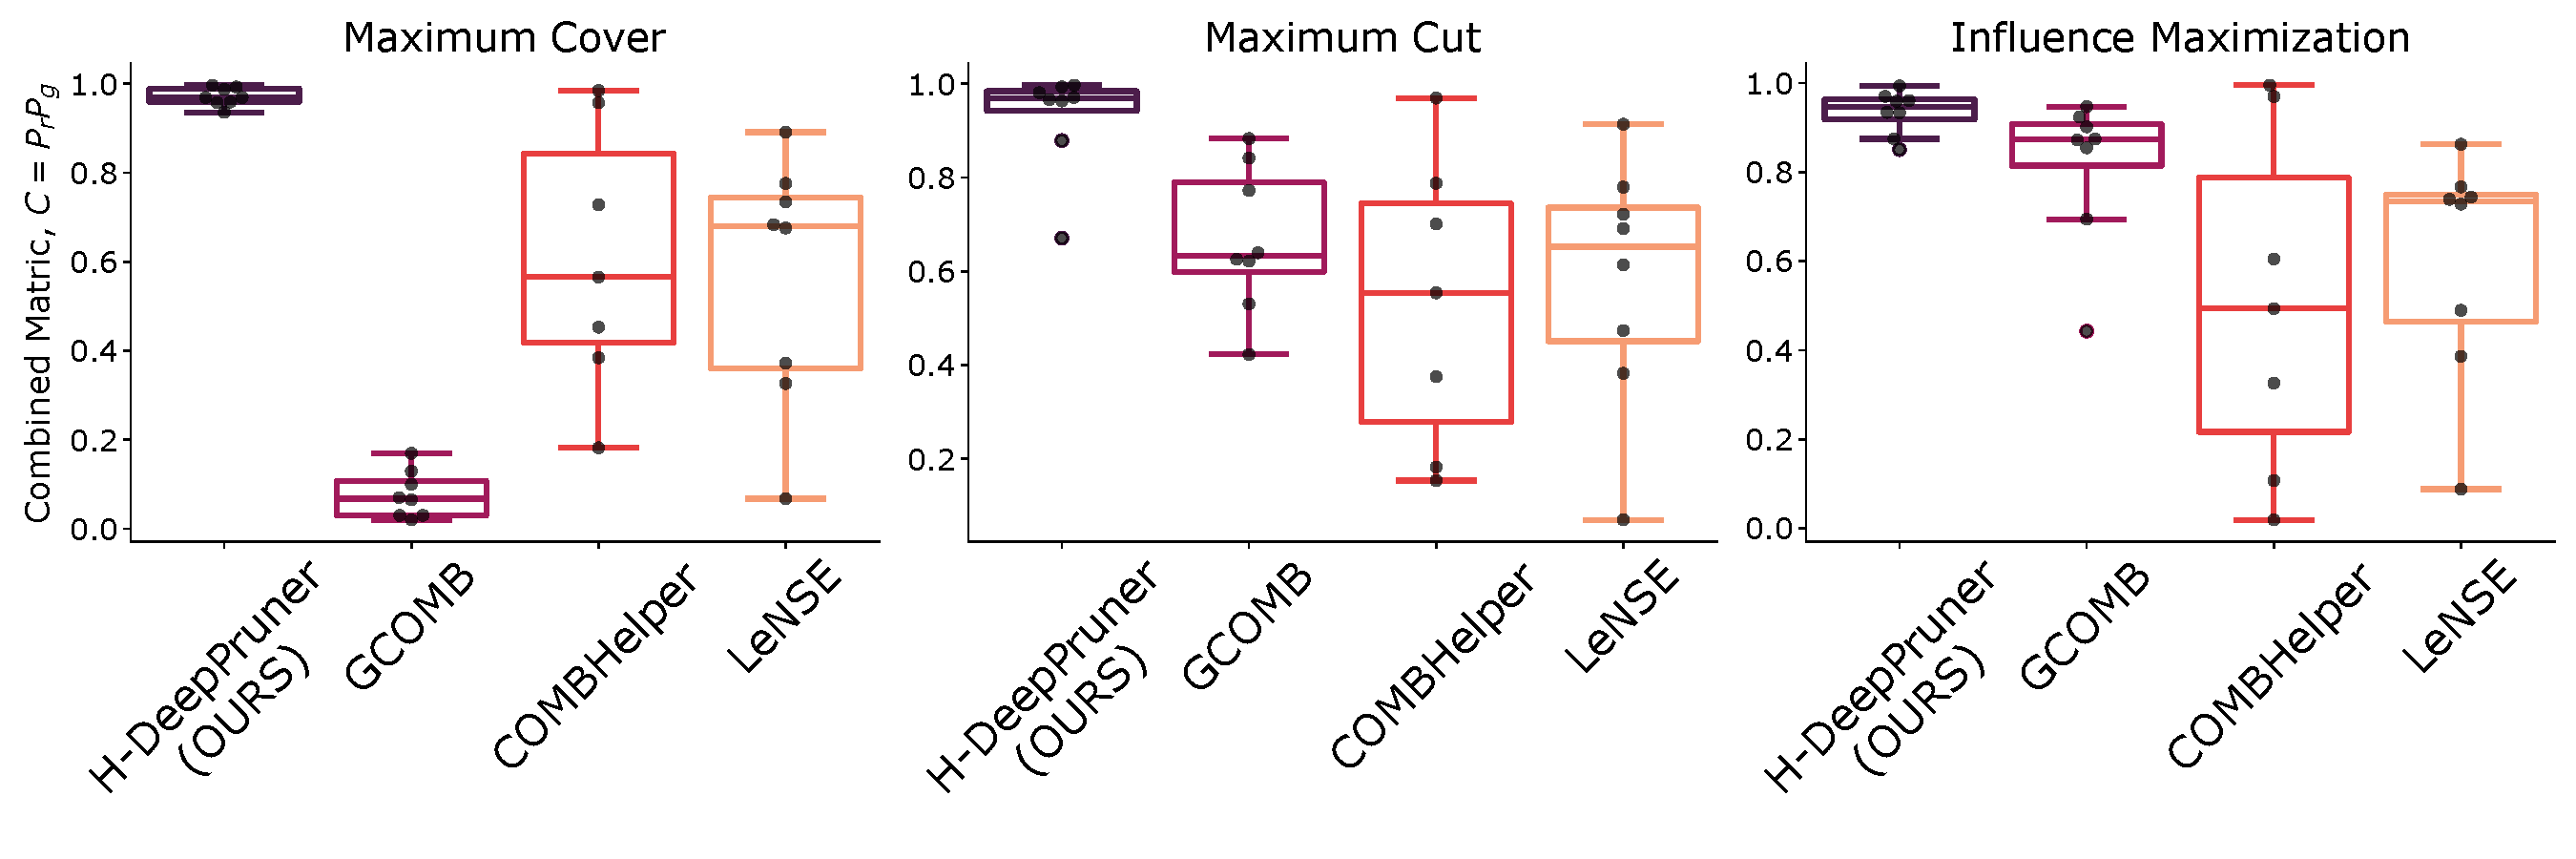
\includegraphics[width=\textwidth]{figures/hdeeppruner/violin_plots.pdf}
  \caption{Box plots of the combined metric (higher is better) for all algorithms across
    all problems. H-DeepPruner consistently achieves the highest combined metric.}
  \label{fig:hdp-violin}
\end{figure}

\subsection{Speed-up Analysis}

Beyond solution quality, effective pruning also accelerates the downstream heuristic by
reducing the size of the input it must process. We measure speed-up as
$S = \text{time}_{\mathcal{U}} / (\text{time}_{\mathcal{U}'} +
\text{time}_{\text{prune}})$, which accounts for both the heuristic runtime on the pruned
set and the pruning time itself. H-DeepPruner accelerates heuristics by up to
40$\times$ by pruning a large fraction of the ground set. The largest speed-ups are
observed on larger graphs where the reduction in ground set size has the most impact on
heuristic runtime. Figure~\ref{fig:hdp-speedup} shows the relative speed-up across all
datasets for MaxCover.

\begin{figure}[t]
  \centering
  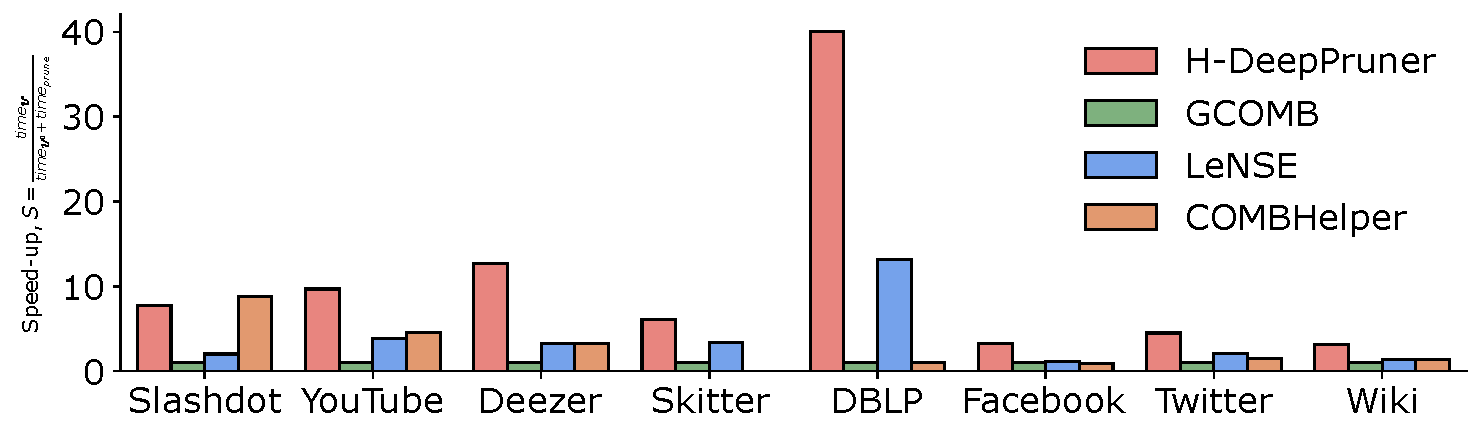
\includegraphics[width=0.7\textwidth]{figures/hdeeppruner/speed_up.pdf}
  \caption{Relative speed-up of using the heuristic on the pruned ground set for all
    algorithms across different datasets for Maximum Cover.}
  \label{fig:hdp-speedup}
\end{figure}

\subsection{Multi-Budget Analysis}

We investigate whether the ground set provided by H-DeepPruner for budget $k = 100$ also
yields close-to-optimal results for lower budgets. Table~\ref{tab:hdp_multibudget} reports
the pruning approximation ratio $P_r$ for budgets 1, 10, 25, 50, 75, and 100 on the IM
problem. In most cases, the ground set provided by H-DeepPruner is also close-to-optimal
for budgets lower than those for which the agent is trained. Values of $P_r > 1$ indicate
that the heuristic achieves a better solution on the pruned ground set than on the full
ground set.

\begin{table}[t]
\centering
\caption{Pruning approximation ratio $P_r$ for IM at various budgets, using the ground set
  produced by H-DeepPruner trained at budget $k = 100$.}
\label{tab:hdp_multibudget}
\resizebox{0.85\textwidth}{!}{%
\begin{tabular}{@{}l cccccc@{}}
\toprule
Graph & $k=1$ & $k=10$ & $k=25$ & $k=50$ & $k=75$ & $k=100$ \\
\midrule
Facebook  & 1.084 & 0.990 & 0.978 & 0.955 & 0.932 & 0.966 \\
Wiki      & 1.063 & 1.014 & 1.001 & 1.011 & 0.968 & 0.969 \\
Deezer    & 0.948 & 0.928 & 0.967 & 0.986 & 0.985 & 0.996 \\
Slashdot  & 1.011 & 1.057 & 0.961 & 0.976 & 1.019 & 0.986 \\
Twitter   & 1.024 & 0.990 & 0.950 & 0.976 & 0.982 & 0.918 \\
DBLP      & 0.615 & 0.659 & 0.763 & 0.810 & 0.852 & 0.835 \\
YouTube   & 1.034 & 1.005 & 1.022 & 0.992 & 0.957 & 0.958 \\
Skitter   & 0.980 & 1.042 & 0.962 & 0.995 & 0.929 & 0.949 \\
\bottomrule
\end{tabular}%
}
\end{table}

\subsection{Ablation Study}

To understand the contribution of each component, we conduct an ablation study comparing
the GNN-only variant (Stage 1 alone) against the full H-DeepPruner pipeline (Stage 1 +
Stage 2). Table~\ref{tab:hdp_ablation} shows that both components are essential for strong
performance, but they contribute in complementary ways. The GNN alone achieves high
pruning approximation ratios ($P_r$ close to 1.0) but moderate pruned fractions ($P_g$
around 0.77--0.86), meaning it preserves solution quality well but does not prune
aggressively enough. Adding NMCTS increases $P_g$ substantially (often to 0.95--1.0)
while only slightly reducing $P_r$, resulting in much higher combined metrics. For
example, on Deezer-MaxCover, the GNN alone achieves $C = 0.763$ while H-DeepPruner
achieves $C = 0.993$. The utility of the GNN pre-pruning step is more pronounced on
larger instances, where running NMCTS on the full ground set would be computationally
infeasible --- the GNN reduces the search space to a manageable size for NMCTS to
operate effectively.

\begin{table}[t]
\centering
\caption{Ablation study: combined metric $C$ for GNN-only versus the full H-DeepPruner
  (GNN + NMCTS) on the SNAP datasets for budget $k = 100$.}
\label{tab:hdp_ablation}
\resizebox{\textwidth}{!}{%
\begin{tabular}{@{}l ccc ccc ccc ccc ccc ccc@{}}
\toprule
& \multicolumn{6}{c}{\textbf{Maximum Cover}} & \multicolumn{6}{c}{\textbf{Maximum Cut}} & \multicolumn{6}{c}{\textbf{Influence Maximization}} \\
\cmidrule(lr){2-7}\cmidrule(lr){8-13}\cmidrule(lr){14-19}
& \multicolumn{3}{c}{GNN} & \multicolumn{3}{c}{H-DeepPruner} & \multicolumn{3}{c}{GNN} & \multicolumn{3}{c}{H-DeepPruner} & \multicolumn{3}{c}{GNN} & \multicolumn{3}{c}{H-DeepPruner} \\
\cmidrule(lr){2-4}\cmidrule(lr){5-7}\cmidrule(lr){8-10}\cmidrule(lr){11-13}\cmidrule(lr){14-16}\cmidrule(lr){17-19}
Graph & $P_r$ & $P_g$ & $C$ & $P_r$ & $P_g$ & $C$ & $P_r$ & $P_g$ & $C$ & $P_r$ & $P_g$ & $C$ & $P_r$ & $P_g$ & $C$ & $P_r$ & $P_g$ & $C$ \\
\midrule
Facebook  & 0.997 & 0.779 & 0.777 & 0.985 & 0.950 & 0.936 & 1.000 & 0.765 & 0.765 & 0.977 & 0.900 & 0.879 & 1.009 & 0.456 & 0.460 & 0.933 & 0.938 & 0.874 \\
Wiki      & 1.000 & 0.863 & 0.863 & 0.997 & 0.961 & 0.958 & 1.000 & 0.864 & 0.864 & 0.998 & 0.969 & 0.966 & 0.979 & 0.766 & 0.750 & 0.964 & 0.969 & 0.934 \\
Deezer    & 1.000 & 0.763 & 0.763 & 0.997 & 0.995 & 0.993 & 1.000 & 0.754 & 0.754 & 0.998 & 0.995 & 0.993 & 1.006 & 0.411 & 0.413 & 0.965 & 0.995 & 0.961 \\
Slashdot  & 1.000 & 0.857 & 0.857 & 0.990 & 0.997 & 0.987 & 1.000 & 0.857 & 0.857 & 1.000 & 0.997 & 0.997 & 0.988 & 0.749 & 0.740 & 0.997 & 0.996 & 0.994 \\
Twitter   & 1.000 & 0.852 & 0.852 & 0.972 & 0.997 & 0.969 & 1.000 & 0.852 & 0.852 & 0.974 & 0.997 & 0.971 & 1.010 & 0.684 & 0.691 & 0.961 & 0.998 & 0.959 \\
DBLP      & 1.000 & 0.790 & 0.790 & 0.969 & 0.999 & 0.969 & 1.000 & 0.797 & 0.797 & 0.964 & 0.999 & 0.963 & 1.002 & 0.515 & 0.516 & 0.853 & 0.999 & 0.850 \\
YouTube   & 1.000 & 0.844 & 0.844 & 0.997 & 1.000 & 0.997 & 1.000 & 0.855 & 0.855 & 0.981 & 1.000 & 0.981 & 0.949 & 0.659 & 0.625 & 0.933 & 1.000 & 0.932 \\
Skitter   & 1.000 & 0.863 & 0.863 & 0.959 & 1.000 & 0.959 & 1.000 & 0.999 & 0.999 & 0.993 & 0.671 & 0.667 & 0.993 & 0.605 & 0.601 & 0.883 & 1.000 & 0.883 \\
\bottomrule
\end{tabular}%
}
\end{table}